
\documentclass[preprint,11pt]{elsarticle}


\usepackage{fullpage} % Package to use full page
\usepackage{parskip} % Package to tweak paragraph skipping
\usepackage{tikz} % Package for drawing
\usepackage{amsmath}
\usepackage{hyperref}
\usepackage{xcolor}
\usepackage{listings}
\usepackage{multicol}

\journal{PEC1}
\begin{document}
\begin{frontmatter}

    \title{Pec1: Temas M1-M2-M3}
    \author{Marc brunet presas}
    \address{Manresa, Barcelona,}
    \begin{abstract}
    Esta primera PEC consiste en una aproximación al mundo GNU/Linux, siguiendo los contenidos marcados en el primer módulo de la asignatura. En ella, deberemos reflexionar sobre los diferentes tipos de distribución y hacer una serie de instalaciones.

    \end{abstract}
\end{frontmatter}


%% main text
\section{Ejercicio 1}
\label{S:1}
Para esta pregunta es necesario documentarse sobre la distribución Debian, Fedora y Suse.
\subsection{Realizar una comparativa entre las licencias de usuario final (EULA) de estas distribuciones que pueden presentar por ejemplo en forma de tabla. Qué conclusiones pueden obtener de esta comparación y cuale son las posibles consecuencias?}

\begin{tabular}{ |p{5cm}||p{2cm}|p{2cm}|p{2cm}|  }
 \hline
 \multicolumn{4}{|c|}{distributions} \\
 \hline
  &Debian &Fedora &Suse\\
 \hline
Componentes no libres  &si &si &-\\
Pagamentos de código fuente &no &si &-\\
Pagamentos de descarga &no &no &si\\
Soporte  &comunidad  &comunidad  &si \\
 \hline
\end{tabular}
\bigskip 

Al analizar un poco las licencias de cada uno de los sistemas vemos que algunos son mantenidos i gestionados totalmente por una comunidad como Debian,  Otros como Fedora i Suse con una empresa privada detrás para obtener beneficio dando soporte o como en una empresa tradicional, vendiendo sus productos y manteniéndolos.


\newpage
\subsection{Analizar las páginas web de las tres distribuciones. Definir en forma precisa cual es el objetivo de cada distribución y que servicios se están ofreciendo a sus usuarios}
\label{S:2}

\paragraph{Debian}\footnote{https://www.debian.org/} sistema operativo conocido por la poca facilidad i las ultimas novedades,  pagina web muy identificativa de esta mentalidad muy esquemática con toda la información en la pagina principal, también los enlaces a las descargas de las ultimas versiones del sistema. Una pagina muy encarada a la funcionalidad i a los usuarios mas experimentados.

\paragraph{Fedora}\footnote{https://getfedora.org/}pagina con estética moderna i con información de las versiones disponibles, separan en 3 versiones para Workstation o personal, server para el uso con servidores o centros de datos, i atom versión muy minimalista para montar servicios basados en contenedores, también muestran imágenes ARM, para usar en dispositivos enveded para IOT o micro ordenadores, muestran una imagen de un producto muy completo i disponible para todas las plataformas o caso de uso.\bigskip

Workstation: versión diseñada para el uso diario profesional o personal, con herramientas para facilitar el trabado i entornos visuales agradables i fáciles de usar con tecnologías de virtualización i docker\bigskip

Server: ofrecen diversas versiones con diversos ciclos de vida para adaptarse despacio o rápidamente a los cambios, usado Modularity para gestionar los ciclos de vida independientemente por paquete, i herramientas de administración i bases de datos\bigskip

Atom: es una versión muy reducida diseñada expresamente para  LDK (Linux-Docker-Kubernetes)\bigskip

\paragraph{Suse}\footnote{https://www.suse.com} página de estilo corporativa da la sensación de vender un producto con una empresa detrás, ofrece servicios de atención al cliente desde la primera página, con información de usos de usos de sus productos, un blog informativo y caso de éxito de sus productos. Dispone de un catalogo de productos ordenado por necesidades para poder ofrecerte el producto más interesante, vende sus productos por versiones Y son extensibles por paquetes, dispone de versiones para el Workstation o personal asta la implementación en la nube, pasado por almacenamiento o gestión de las infraestructuras en la empresa, Están muy encarados a sistemas para empresas. \bigskip

\subsection{A partir de esta información proponga tres situaciones de instalación en las cuales aconsejaría utilizar una de estas distribuciones justificando de forma razonada esta propuesta}\bigskip

depures de analizar un poco cada una de les distribuciones recomendaría suse para una empresa que está en planeando una migración de Windows o mac os x , ja que dispone de características muy parecidas, como un puesto de respuesta y resolución de problema, seguramente tendería un sistema de orientación y acompañamiento en la migración, aparte dispone productos para todas las necesidades en una sola compañía, seria una migración completa en todos los aspectos desde los departamentos más tecnológicos asta los más administrativos, ofreciendo respuesta a los departamentos de IT en la gestión y mantenimiento de la maquinas, a los desarrolladores en el sistema operativo y en los administradores en el aspecto gráfico y sus herramientas de ofimáticas.\bigskip

Fedora lo recomendaría en una empresa tecnológica que este planeado un migración ofrece sistemas Workstation y servers con la posibilidad de ir a los microservicios, tendrían que ser una empresa con mentalidad moderna y con un objetivo de modernización en sus planes de futuro, tendrán que estar modernizado el software constantemente sin un soporte oficial i deberán apoyarse de la comunidad, teniendo opciones de dejar parte del sistema en una versión antigua. La parte más tecnológica de la empresa no tendrá problemas pero la parte más administrativa puede tener algún problema de compatibilidad i tendrá que solucionarlo la parte más tecnología pero tanto puede plantearse una migración parcial\bigskip

Debian solo lo recomendaría en usuaria avanzados todo i que te una parte estable puede ser bastate complicado una actualización o inhalación, seria una migración solo de la parte mas tecnología de la empresa incluso solo los servidores en algún caso o también los miembros de IT i desarrolladores\bigskip

\subsection{ Comentar para cada una de ella y de la información previa el rango de uso de cada distribución (se puede seguir el formato tal y como aparece en la página de Distrowatch pero debe ser elaborado con la información previa que han analizado.}\bigskip


\begin{tabular}{ |p{4cm}||p{3cm}|p{3cm}|p{3cm}|  }
 \hline
 \multicolumn{4}{|c|}{distributions} \\
 \hline
  &Workstation  &Server  &Cloud \\
 \hline
Debian &si &si &si\\
Fedora Workstation  &si &no &no\\
Fedora Server &no &si &si\\
Fedora atom &no &si &si \\
suse &si &si &si \\
 \hline
\end{tabular}
\bigskip 

Fedora con las versiones Atom i Server pueden usarse en servidores locales para obtener un servidor local con aplicaciones tradicionales, o contenedores, indistintamente, todo i que cada versión esta más encara da cada uso particular.\bigskip

Devian como tal puede usarse indistintamente en cualquier parte pero la complicación de no disponer de una versión especifica puede complicar las tareas de configuración i instalación de los entornos.\bigskip

Suse puede usarse en todos los entornos dispone versiones especificas para cada uso y extensibles con paquetes extras, lo que lo hace perfectamente adaptable a cada uso.\bigskip

\clearpage
\section{Ejercicio 2}
Para esta parte práctica, se deberá hacer al menos dos instalaciones de GNU/Linux, en una configuración de escritorio (no pensado para servidor) y con un mismo gestor de ventanas en los dos casos (Gnome, KDE, o el que deseen – pero que sea el mismo en todas las instalaciones). Se deberán de entre las siguientes tres posibles ramas: Fedora/CentOS, Debian/Ubuntu o Suse. Para algunas distribuciones pueden usar el material distribuido con la asignatura, descargar otras imágenes directamente desde Internet oaprovechar material que ya tengan disponible. En todo caso, habra que usar imágenes de CD/DVD de instalación, y no una imagen completa de sistema ya preparada por su ejecución.\bigskip

\subsection{Documentar el proceso de instalación: qué diferencias mayores han encontrado en el software para hacer la instalación, qué problemas han detectado (dispositivos que no funcionan, resolución, etc) y qué soluciones han buscado y aplicado. Como muestra del funcionamiento de deberá mostrar en un terminal la ejecución de comando uname -a y se debe mostrar que pueden navegar a una página de Internet actualizada (donde se indique claramente la fecha y hora, por ejemplo a un diario) }

Realizado y documentado en el anexo, Todo y que en la inhalación de los sistemas Ubuntu 18.04 y Fedora Workstation 29 no he tendió problemas con ningún adaptador ni dispositivo cuando he instalado Ubuntu en algún portátil he tenido problemas con las tarjetas gráfica Nvidia y algunos adaptadores de Wifi nada que con descargase los controladores adicionales públicos o privativos no pudiera solucionar o reconfigurar parte del sistema.

\subsection{Examinar el sistema de ficheros y realizar una tabla comparativa de: qué diferencias han detectado entre las dos instalaciones? Qué ocupación del disco tienen – y, si hay variaciones, como las pueden explicar?} 
\footnote{Son dos maquinas diferentes, ja que tengo 2 en el ordenador del trabado y 2 en el personal} Comparamos las estructuras de ficheros con un tree -L 2 / 

\begin{tabular}{ |p{7cm}||p{7cm}| }
    \hline
    \multicolumn{2}{|c|}{Diferencias} \\
    \hline
    Ubuntu& Fedora\\
    \hline
   	bin   & bin -\textgreater  usr/bin   \\
    grub &   grub2 \\
    libX & libX-\textgreater usr/libX\\
    sbin & sbin-\textgreater usr/sbin\\
    469 directories, 680 files & 	483 directories, 360 files \\
    \hline
\end{tabular}

Ja podemos observar que la gestión del /bin /lib / lib64 y /sbin es diferente, Ubuntu tira más de la carpeta como tal y en Fedora tienen enlaces simbólicos a las carpetas de /usr donde tiene los ficheros, Ubuntu los tiene divididos en las dos, comento el Grupb ja que Ubuntu tiene más paquetes y a una versión anterior a los que integra Fedora, podemos observar algunas diferencias más, como que en /var Fedora tiene más directorios o que en general tiene menos ficheros. \bigskip

Comprobación del uso del disco de Febdora y Ubuntu actualizados en día 31/10/2018:
\begin{lstlisting}[ basicstyle=\tiny,]
    [marc@localhost ~]$ df -h
    S. fitxers               Mida En ús Lliure  %Ús Muntat a
    devtmpfs                 972M     0   972M   0% /dev
    tmpfs                    985M  4,0K   985M   1% /dev/shm
    tmpfs                    985M  2,5M   983M   1% /run
    tmpfs                    985M     0   985M   0% /sys/fs/cgroup
    /dev/mapper/fedora-root   17G  5,2G    11G  33% /
    tmpfs                    985M  164K   985M   1% /tmp
    /dev/sda1                976M  146M   764M  16% /boot
    tmpfs                    197M  2,3M   195M   2% /run/user/981
    tmpfs                    197M   12M   186M   6% /run/user/1000
    /dev/sr0                 1,8G  1,8G      0 100% /run/media/marc/Fedora-WS-Live-29-1-2

\end{lstlisting}

\begin{lstlisting}[ basicstyle=\tiny,]
    (marc@ubuntu:~$ df -h
    Filesystem      Size  Used Avail Use% Mounted on
    udev            453M     0  453M   0% /dev
    tmpfs            97M  3.0M   94M   4% /run
    /dev/sda1        20G  5.2G   14G  28% /
    tmpfs           482M     0  482M   0% /dev/shm
    tmpfs           5.0M  4.0K  5.0M   1% /run/lock
    tmpfs           482M     0  482M   0% /sys/fs/cgroup
    /dev/loop0       87M   87M     0 100% /snap/core/4917
    /dev/loop1       35M   35M     0 100% /snap/gtk-common-themes/319
    /dev/loop2      141M  141M     0 100% /snap/gnome-3-26-1604/70
    /dev/loop3      2.4M  2.4M     0 100% /snap/gnome-calculator/180
    /dev/loop4       13M   13M     0 100% /snap/gnome-characters/103
    /dev/loop5       15M   15M     0 100% /snap/gnome-logs/37
    /dev/loop6      3.8M  3.8M     0 100% /snap/gnome-system-monitor/51
    tmpfs            97M   16K   97M   1% /run/user/121
    tmpfs            97M   48K   97M   1% /run/user/1000

\end{lstlisting}
Podemos observar que el uso de disco no es tan diferente los dos consumen unos 5,2GB en el /, que es la raíz principal sel sistema, vemos que ubuntu usa los dispositivos loop para acceder a ficheros como dispositivo de bloques 

\subsection{También incluir en esta tabla si se han creado los mismos usuarios y grupos? Examinar el contenido de los ficheros /etc/passwd y /etc/group, así como los derechos de acceso de los ficheros de configuración (en el directorio /etc) y extraer conclusiones.}

Las salidas de los comandos cat /etc/passwd y cat /etc/group en el anexo, para poder observar alguna diferencia vamos a ver que es cada valor de la salida:
\begin{lstlisting}[ basicstyle=\tiny,]
root:x:0:0:root:/root:/bin/bash\newline
marc:x:1000:1000:marc,,,:/home/marc:/bin/bash
\end{lstlisting}
root es el nombre de usuario, el siguiente valor es la contraseña x significa que esta enchipada y guardada en /etc/shadow file, los siguientes valores son el userID y el grupID, un comentario y el Home del usuario y la terminal

Tenemos una lista de usuarios comunes todo y que en grupos o IDs diferentes cuando veamos el /etc/group veremos si se comportan de forma diferente, todo y que puede ser los mismos creados de forma diferente, aparte tenemos que Fedora dispone de más usuarios directamente algunos preparados para algún servicio o concreto como FTP, OpenVPN o Apache entre otros

\textbf{/etc/passwd}
\begin{lstlisting}[ basicstyle=\tiny,]
root:x:0:0:root:/root:/bin/bash
bin:x:2:2:bin:/bin:/usr/sbin/nologin
daemon:x:1:1:daemon:/usr/sbin:/usr/sbin/nologin
sync:x:4:65534:sync:/bin:/bin/sync
mail:x:8:8:mail:/var/mail:/usr/sbin/nologin
marc:x:1000:1000:marc,,,:/home/marc:/bin/bash
systemd-network:x:100:102:systemd Network
systemd-resolve:x:101:103:systemd
gdm:x:121:125:Gnome Display Manager:/var/lib/gdm3:/bin/false
games:x:5:60:games:/usr/games:/usr/sbin/nologin
Management,,,:/run/systemd/netif:/usr/sbin/nologin
lp:x:7:7:lp:/var/spool/lpd:/usr/sbin/nologin
colord:x:117:123:colord colour management daemon,,,:/var/lib/colord:/usr/sbin/nologin
nobody:x:65534:65534:nobody:/nonexistent:/usr/sbin/nologin
gnome-initial-setup:x:120:65534::/run/gnome-initial-setup/:/bin/false
rtkit:x:109:114:RealtimeKit,,,:/proc:/usr/sbin/nologin
pulse:x:115:120:PulseAudio daemon,,,:/var/run/pulse:/usr/sbin/nologin
geoclue:x:119:124::/var/lib/geoclue:/usr/sbin/nologin
avahi-autoipd:x:106:112:Avahi autoip daemon,,,:/var/lib/avahi-autoipd:/usr/sbin/nologin
dnsmasq:x:108:65534:dnsmasq,,,:/var/lib/misc:/usr/sbin/nologin
\end{lstlisting}



\textbf{/etc/group}
\begin{multicols}{2}
\begin{lstlisting}[ basicstyle=\tiny,]
root:x:0:
daemon:x:1:
bin:x:2:
sys:x:3:
adm:x:4:syslog,marc
tty:x:5:
disk:x:6:
lp:x:7:
mail:x:8:
kmem:x:15:
cdrom:x:24:marc
man:x:12:
dialout:x:20:
floppy:x:25:
tape:x:26:
video:x:44:
audio:x:29:pulse
users:x:100:
utmp:x:43:
input:x:104:
systemd-journal:x:101:
systemd-network:x:102:
systemd-resolve:x:103:
dip:x:30:marc
rtkit:x:114:
pulse-access:x:121:
pulse:x:120:
geoclue:x:124:
avahi:x:122:
colord:x:123:
gdm:x:125:
marc:x:1000:
\end{lstlisting}
Los grupos se identifican por nombre, password en el mismo caso que los usuarios, grupo ID i lista de usuarios u grupos de usuarios\medskip

Tenemos el mismo caso unos usuarios genéricos similares a los dos pero con el IDs diferentes, aparte podemos observar que Fedora dispone de más grupos muchos de ellos para servicios en concreto, de forma que nos intentan simplificar la faena a la hora de gestionar los permisos en los servicios, la gestión de los grupos también es un poco diferente, en Fedora vemos que los grupos están generalmente vacíos en cambio en Ubuntu tiene más tendencia a asignar grupos a otos grupos o los usuarios directamente, por ejemplo el grupo adm que comparten un Ubuntu está asignado a syslog y a marc, en fedora esta vació
\end{multicols}

\subsection{Extraer conclusiones sobre los diferentes aspectos de cada distribución
después de haber ejecutado por lo menos 20 comandos de los sugeridos en
la documentación del capítulo (Nivel usuario).}


\section{En cada caso, explicar que hacen los siguientes comandos o dar el
comando/s que realiza la acción propuesta: }

\subsection{Imprime por pantalla las líneas que tiene el tercer parámetro o ID más pequeño que 512 o que el cuarto parámetro o ID del grupo mayor que 30,  podríamos cambiar el comando y dejándolo un poco más claro}
\begin{lstlisting}[language=bash]
awk -F: '($3 > 512 || $4 > 30)' /etc/passwd  
\end{lstlisting}

\subsection{Da la hora pero, lo que hacemos es crear un fichero temporal para guardar el comando, cambiarle los permisos y ejecutarlo se podría simplificar con el comando directo}

\subsection{Da la hora pero, lo que hacemos es crear un archivo temporal para guardar el comando, cambiarle los permisos y ejecutarlo, se podría simplificar con el comando directo, le damos los permisos de lectura y ejecución más el S que determina que se ejecuta con el usuario que lo creo, puede ser útil si no queremos dar mayores permisos a un grupo para ejecutar un comando y le preparamos un script para realizar la tarea}

\subsection{}

ordenados por CPU 
\begin{lstlisting}[language=bash,  basicstyle=\tiny,]
top -n 1 -b | awk '/a/ {if(NR>7)print $9"\t"$1"\t"$2}' | head -10 | awk '{print $3"\t"$2"\t"$1}' |
sort > /tmp/cpu;  echo -e "user\tpid\tcpu%" $1; cat /tmp/cpu
\end{lstlisting}

ordenado por Memoria

\begin{lstlisting}[language=bash,  basicstyle=\tiny,]
top -n 1 -b | awk '/a/ {if(NR>7)print $10"\t"$1"\t"$2}' | head -10 | awk '{print $3"\t"$2"\t"$1}' |
sort > /tmp/cpu;  echo -e "user\tpid\tmem%" $1; cat /tmp/cpu

\end{lstlisting}

\subsection{}
\begin{lstlisting}[language=bash,  basicstyle=\tiny,]
ls -lhR /usr  2> /dev/null | awk '{if($3!="")print $5 "\t" $9}' | sort -rh | head -24

\end{lstlisting}

Realismo el las eliminado las rasquetas erróneas normalmente por permisos de lectura del usuario actual filtramos las líneas que no tenga 3r argumento que son las carpetas y re ordenamos las columnas las ordenamos y mostramos las 24 primeras líneas, como dato curio he tirado el comando en la raíz / i ha aparecido un fichero curioso 
\begin{lstlisting}[language=bash,  basicstyle=\tiny,]
[marc@localhost ~]$ ls -lh /proc/kcore
-r--------. 1 root root 128T 5 nov. 06:21 /proc/kcore

\end{lstlisting}
pero es un fichero mágico que guarda punteros de memoria

\subsection{}
\begin{lstlisting}[language=bash,  basicstyle=\tiny,]
ls -lhR /usr  2> /dev/null | awk '{if($2=="") dir=substr($1, 1, length($1)-1);
else print $1 "\t" dir"/"$9}' |  grep '^\S*x\S*'

\end{lstlisting}

\subsection{}
\begin{lstlisting}[language=bash,  basicstyle=\tiny,]
USERADD=$(tail -1 /etc/passwd | awk -F ':' '{if($3+1<2049) print "-u " $3+1 " marc2"; else print "uid > 2048" }');
GRUPADD=$(cat /etc/group | grep users | awk '{if ($1!="") print " -a -G users marc2"; else sudo groupadd users}');
sudo useradd $USERADD; sudo usermod $GRUPADD; unset USERADD; unset GRUPADD 

\end{lstlisting}

\clearpage
\subsection{hacer un análisis de 10 comandos de su elección (no utilizados en los
puntos anteriores) y mostrar su ejecución y para que los han utilizado.}
\begin{multicols}{2}
\textbf{lsusb}: Muestra la información de los puertos USB que tenemos y con -t mostramos información del bus físico, con -v la versión, podríamos añadir -d para ver el fabricante u otras banderas

\textbf{touch} Nos permite crear ficheros vacíos o cambiar los timestamps de un archivo tiene algunas banderas interesantes como -a para cambiar la hora de acceso a un fichero o -t para cambiar la fecha de creación de un fichero entre otras 

\textbf{find}  Busca fichero por el sistema que cumplen unas condiciones que podemos especificar con: -user que especificamos el usuario que nos interesa o -mtime que especificamos los días de la ultima modificación.

\textbf{tar} Nos permite comprimir y descomprimir archivos, tiene muchas opciones de banderas pero las más utilizadas son -cvf que vendría a ser -c create para crear el fichero -v para ver el progreso de compresión y -f el nombre del archivo de destino quedando tar -cvf archive.tar file directory

\textbf{sed} Nos permite procesar ficheros de texto y modificarlos, con ejemplos útiles como sed 's/c1/c2/g' hola.txt cambiamos los c1 del hola.txt a c2, pude ser muy útil para cambiar valores en ficheros grandes o que estén muy repetidos

\textbf{dd} Nos permite convertir y copiar a archivo, permite convertir una área del disco en un archivó con todo su contenido muy útil en copias de seguridad, haremos una copia de hda en bloques de 1M y los comprimimos con gzip, los enviaos por medio de ssh a un host remoto y los guardamos en el fichero hda.gz ejemplo:
\begin{lstlisting}
dd bs=1M if=/dev/hda | gzip |
mid ssh user@ip_addr 'dd of=hda.gz'
\end{lstlisting}

\textbf{ifconfig} Nos permite ver y configurar los adaptadores de red para levantarlos o apagarlos o cambiar algunos parámetros, podemos cambiarles la ip con seccionar el adaptador y a continuación la ip,con netmask cambiamos la mascara de red, entre otras acciones

\textbf{iptables} Nos permite el control de los paquetes, es decir podemos redirecionar los paquetes de una interfaz a otra o de un host a otro, con o sin traducion o bloqueando algún tipo o no

\textbf{whatis} Nos muestra de descripción de un comando por la pantalla

\textbf{apt-get o yum } Nos permiten gestionar los paquetes, podemos instalar o desinstalar paquetes del sistema actualizarlos
\end{multicols}

\clearpage
\section{Escribir un shell script para bash que muestre la actividad de los usuarios y que solo pueda ejecutar el usuario root. La salida será por pantalla y se irá almacenando en un archivo histórico por cada usuario en el directorio /root/informes/usuario-fecha-hora. Los parámetros del script (argumentos en la línea de comandos) serán los siguientes:}

\begin{itemize}
    \item-a presentar un lisatado de los archivos/directorio que cada usuario ha modificado en las últimas 24 horas.
    \item-e Informar sobre el número de conexiones y el tiempo total de conexión acumulado por cada usuario durante la última semana.
    \item-uu usuario Informar solamente sobre el usuario indicado. Si no existe este parámetro, se deberá presentar el informe para cada uno de los usuarios reales del sistema.
\end{itemize}

Incluir el código comentado y los resultados de las pruebas de ejecución.























\clearpage
\section{bibliografía}
    \textbf{URLS:}
    \begin{itemize}
        \item web del proyecto suse https://www.suse.com consulta 30/oct/2018
        \item web del proyecto getfedora https://www.getfedora.org consulta 30/oct/2018
        \item web del proyecto debian  https://www.debian.org consulta 30/oct/2018
        \item Web de consulta de distribuciones https://distrowatch.com consulta 30/oct/2018
    \end{itemize}
























\clearpage
\section{Anex}
\subsection{Ubuntu 18.04}
\begin{figure}[!htbp]
    \begin{center}
        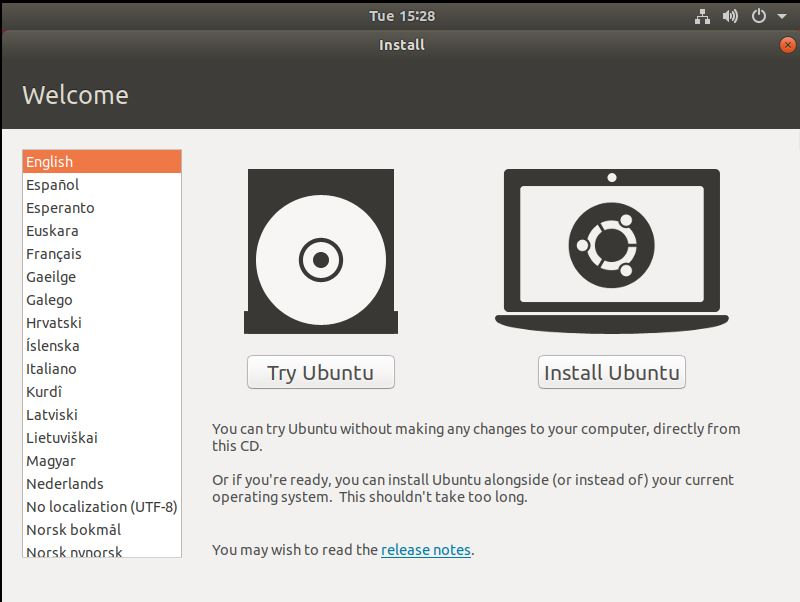
\includegraphics[width=11cm]{anex/ubuntu1.JPG}
    \end{center}
    \caption{Escogemos si lo probamos o lo instalamos y la distribución del teclado}
    \begin{center}
        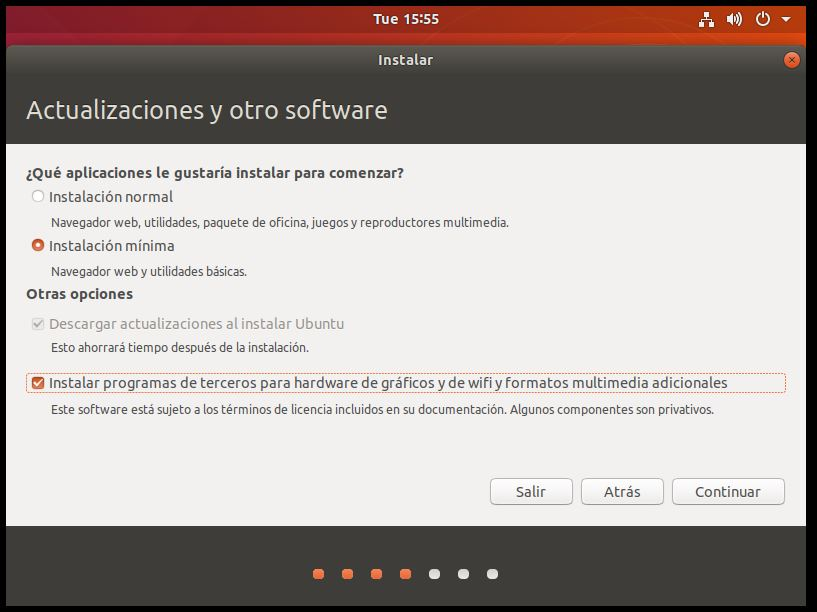
\includegraphics[width=11cm]{anex/ubuntu2.JPG}
    \end{center}
    \caption{Una vez seleccionado el idioma escomeremos la distribución del teclado y procedemos al tipo de instalación que queremos, y si deseamos incluir programas de 3r (que pueden contener licencias privativas)}
\end{figure}
\begin{figure}[!htbp]
    \begin{center}
        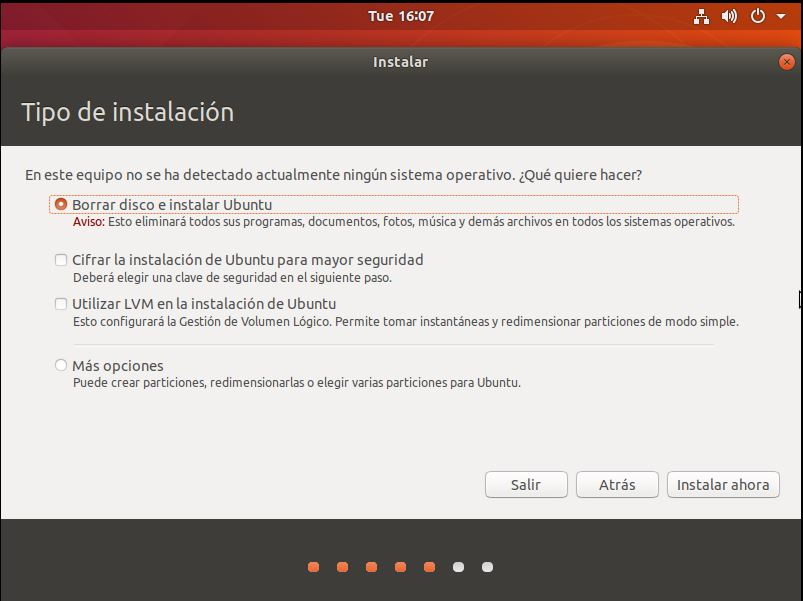
\includegraphics[width=11cm]{anex/ubuntu3.JPG}
    \end{center}
    \caption{Nos permite selección un formateo del disco automático o escoger el formato que no nosotros queremos}
    \begin{center}
        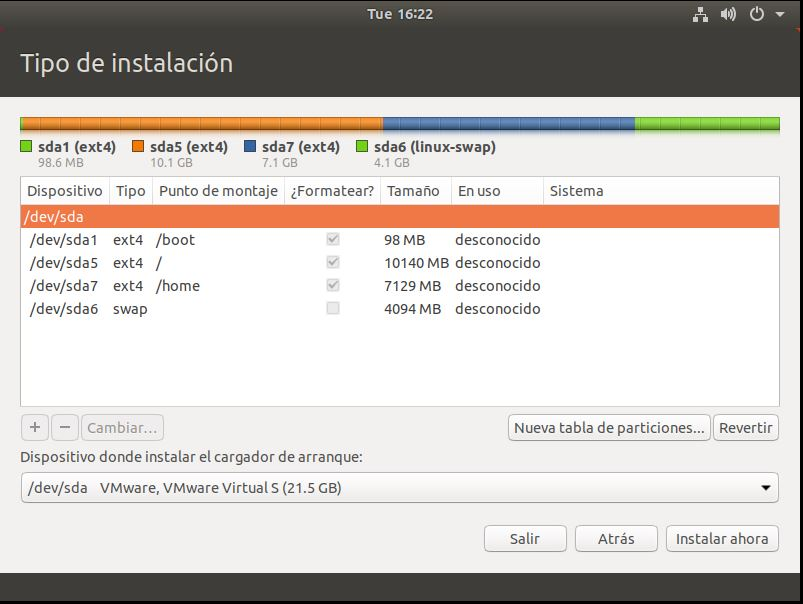
\includegraphics[width=11cm]{anex/ubuntu4.JPG}
    \end{center}
    \caption{Podemos configurar las particiones en el formato que queramos una partición para todo el sistema o frentes particiones para las carpetas generales}
\end{figure}

Haremos unas configuraciones básicas de nombre de usuario y credenciales nombre de maquina y ubicación, y el poseso de instalación seguirá y actualizará la maquina asta que no pida el reinicio

\begin{figure}[!htbp]
    \begin{center}
        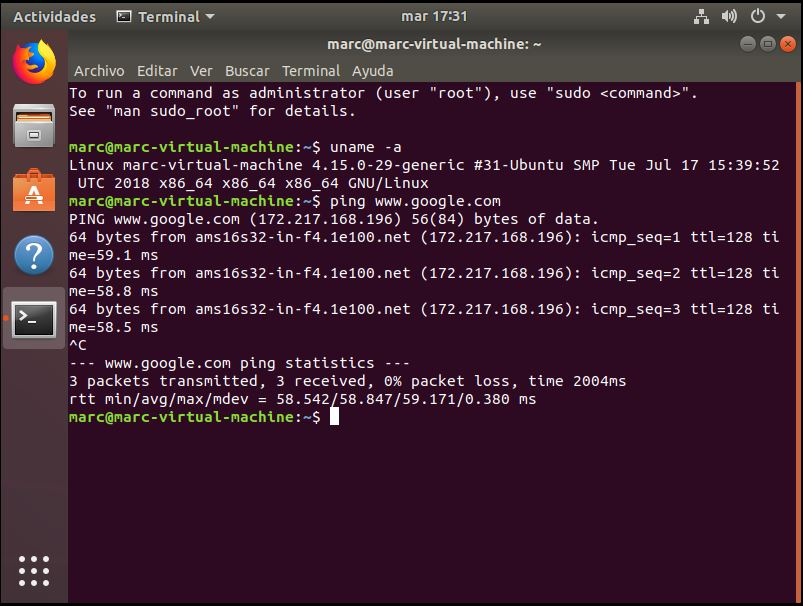
\includegraphics[width=11cm]{anex/ubuntu5.JPG}
    \end{center}
    \caption{,ejecución del comando uname -a y un ping a google.com}
    \begin{center}
        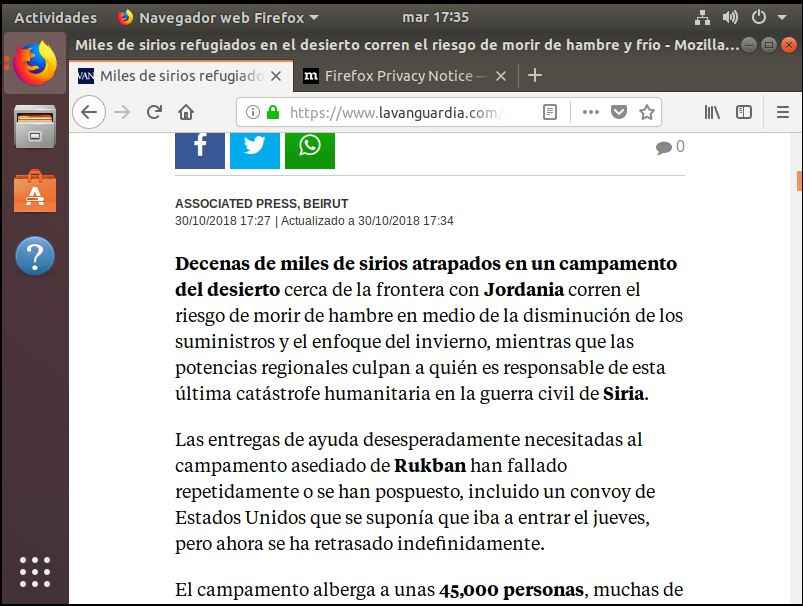
\includegraphics[width=11cm]{anex/ubuntu6.JPG}
    \end{center}
    \caption{comprobación de una noticia de la vanguardia \newline https://www.lavanguardia.com/internacional/20181030/452657349845/siria-campamento-rukban-hambre-frio.html}
\end{figure}

\clearpage
\subsection{Fedora 29}
\begin{figure}[!htbp]
    \begin{center}
        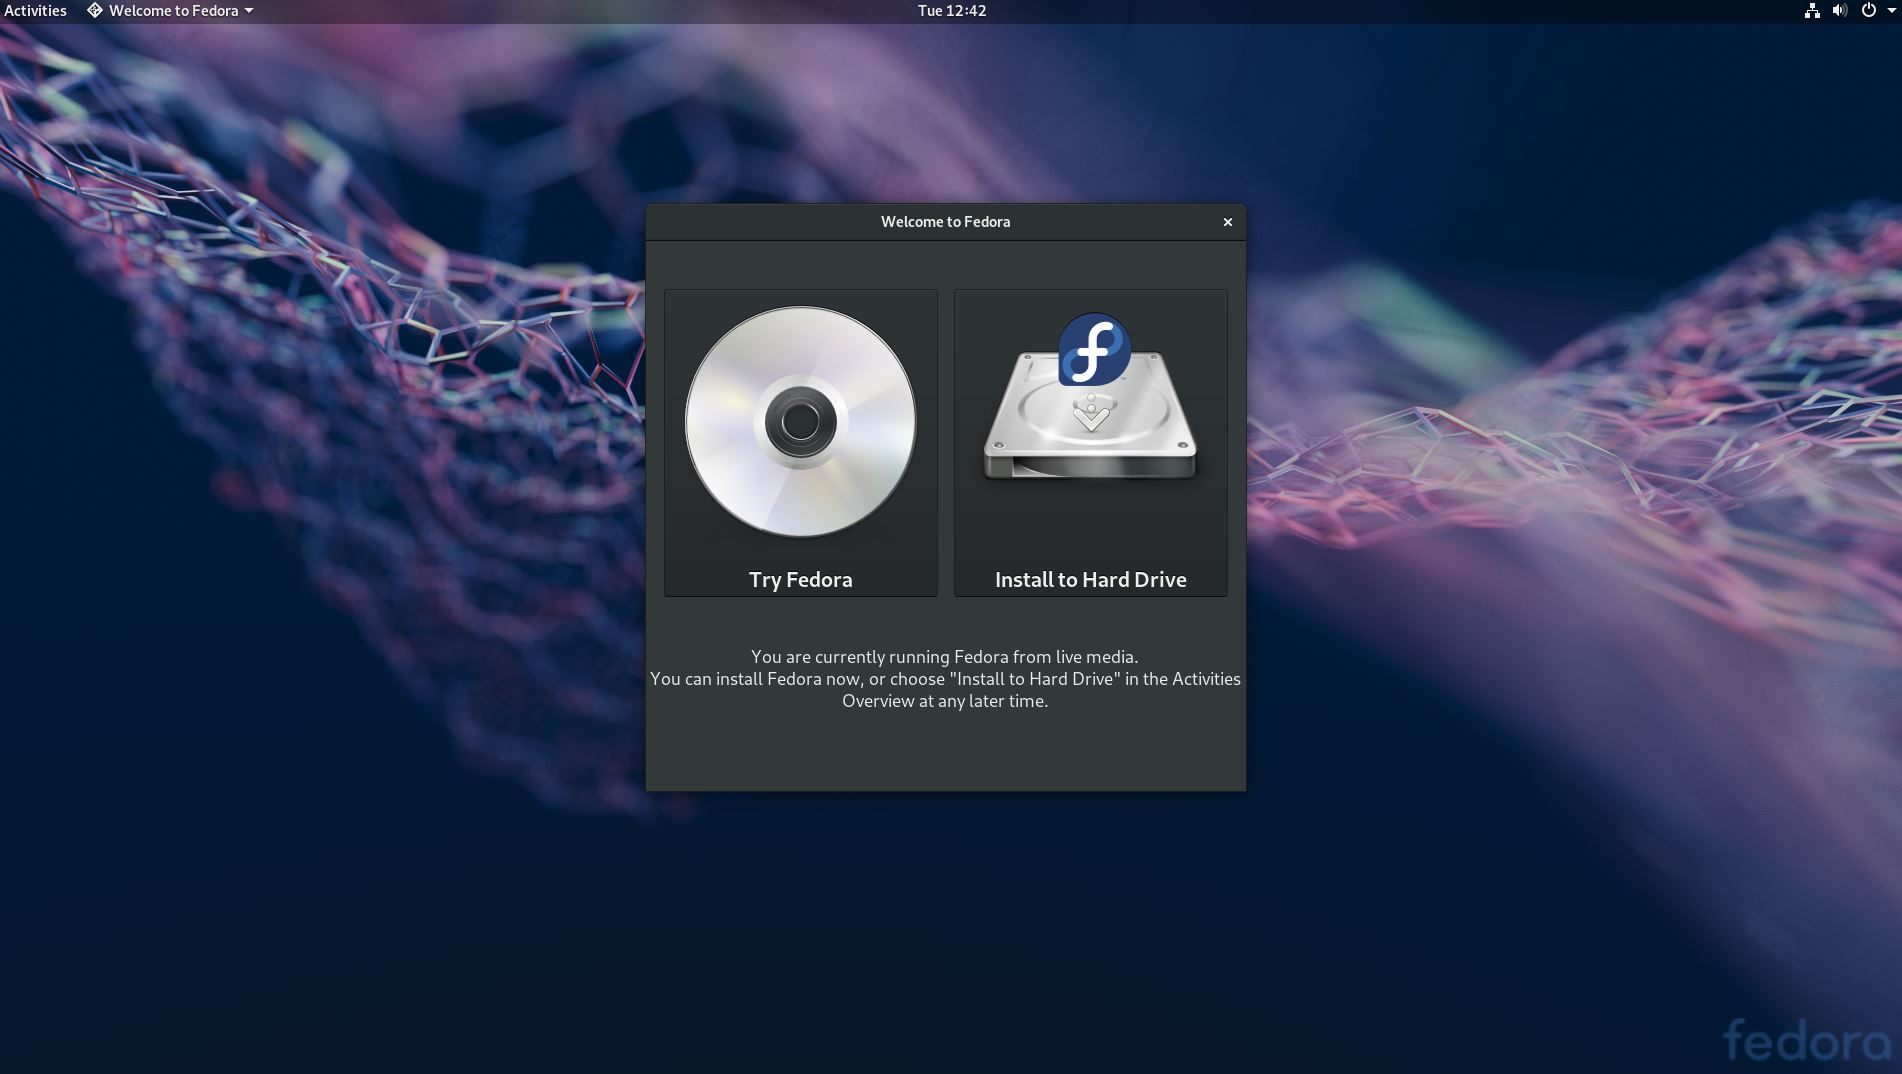
\includegraphics[width=11cm]{anex/fedora1.JPG}
    \end{center}
    \caption{Pantalla inicial de la inhalación de fedroa podemos instalar o probar }
    \begin{center}
        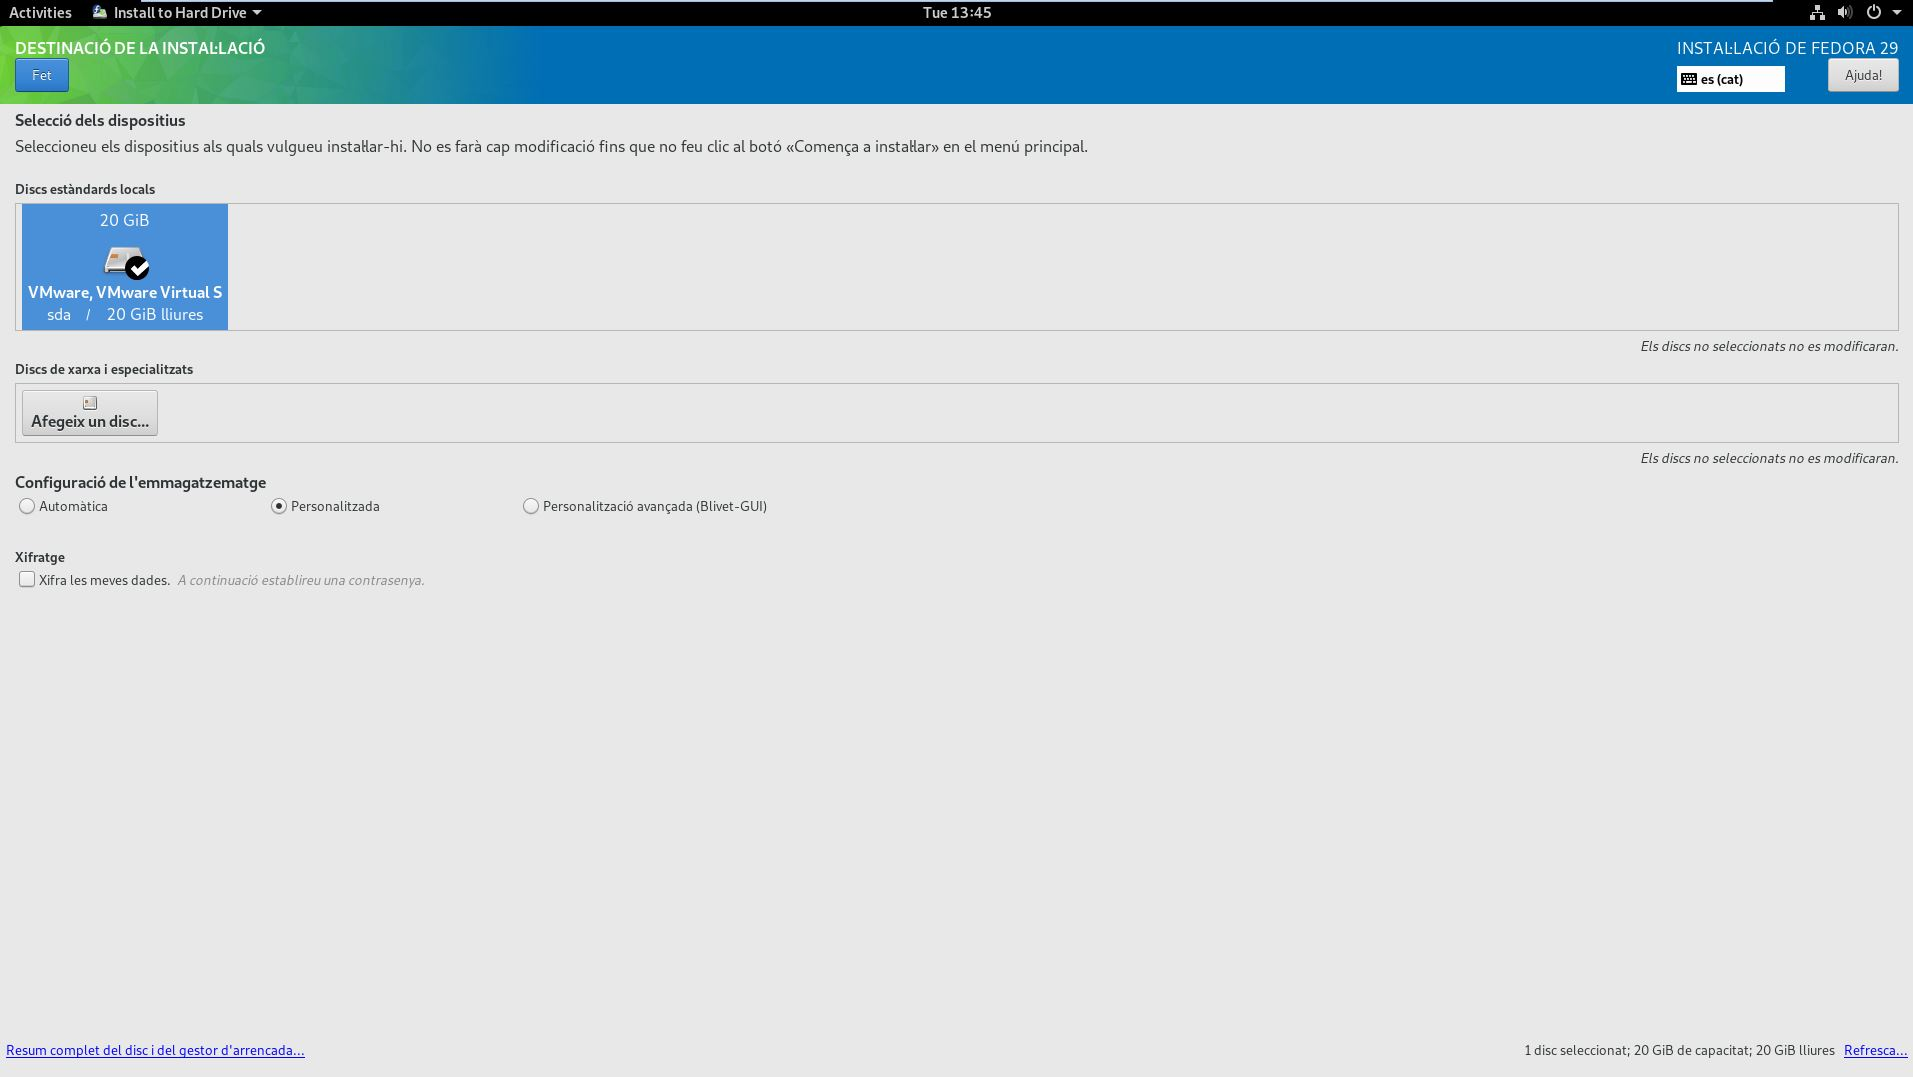
\includegraphics[width=11cm]{anex/fedora2.JPG}
    \end{center}
    \caption{Configuración del disco podemos dejarlo en automático personalizado vamos a realizar la misma configuración que con el ubuntu}
\end{figure}
\begin{figure}[!htbp]
    \begin{center}
        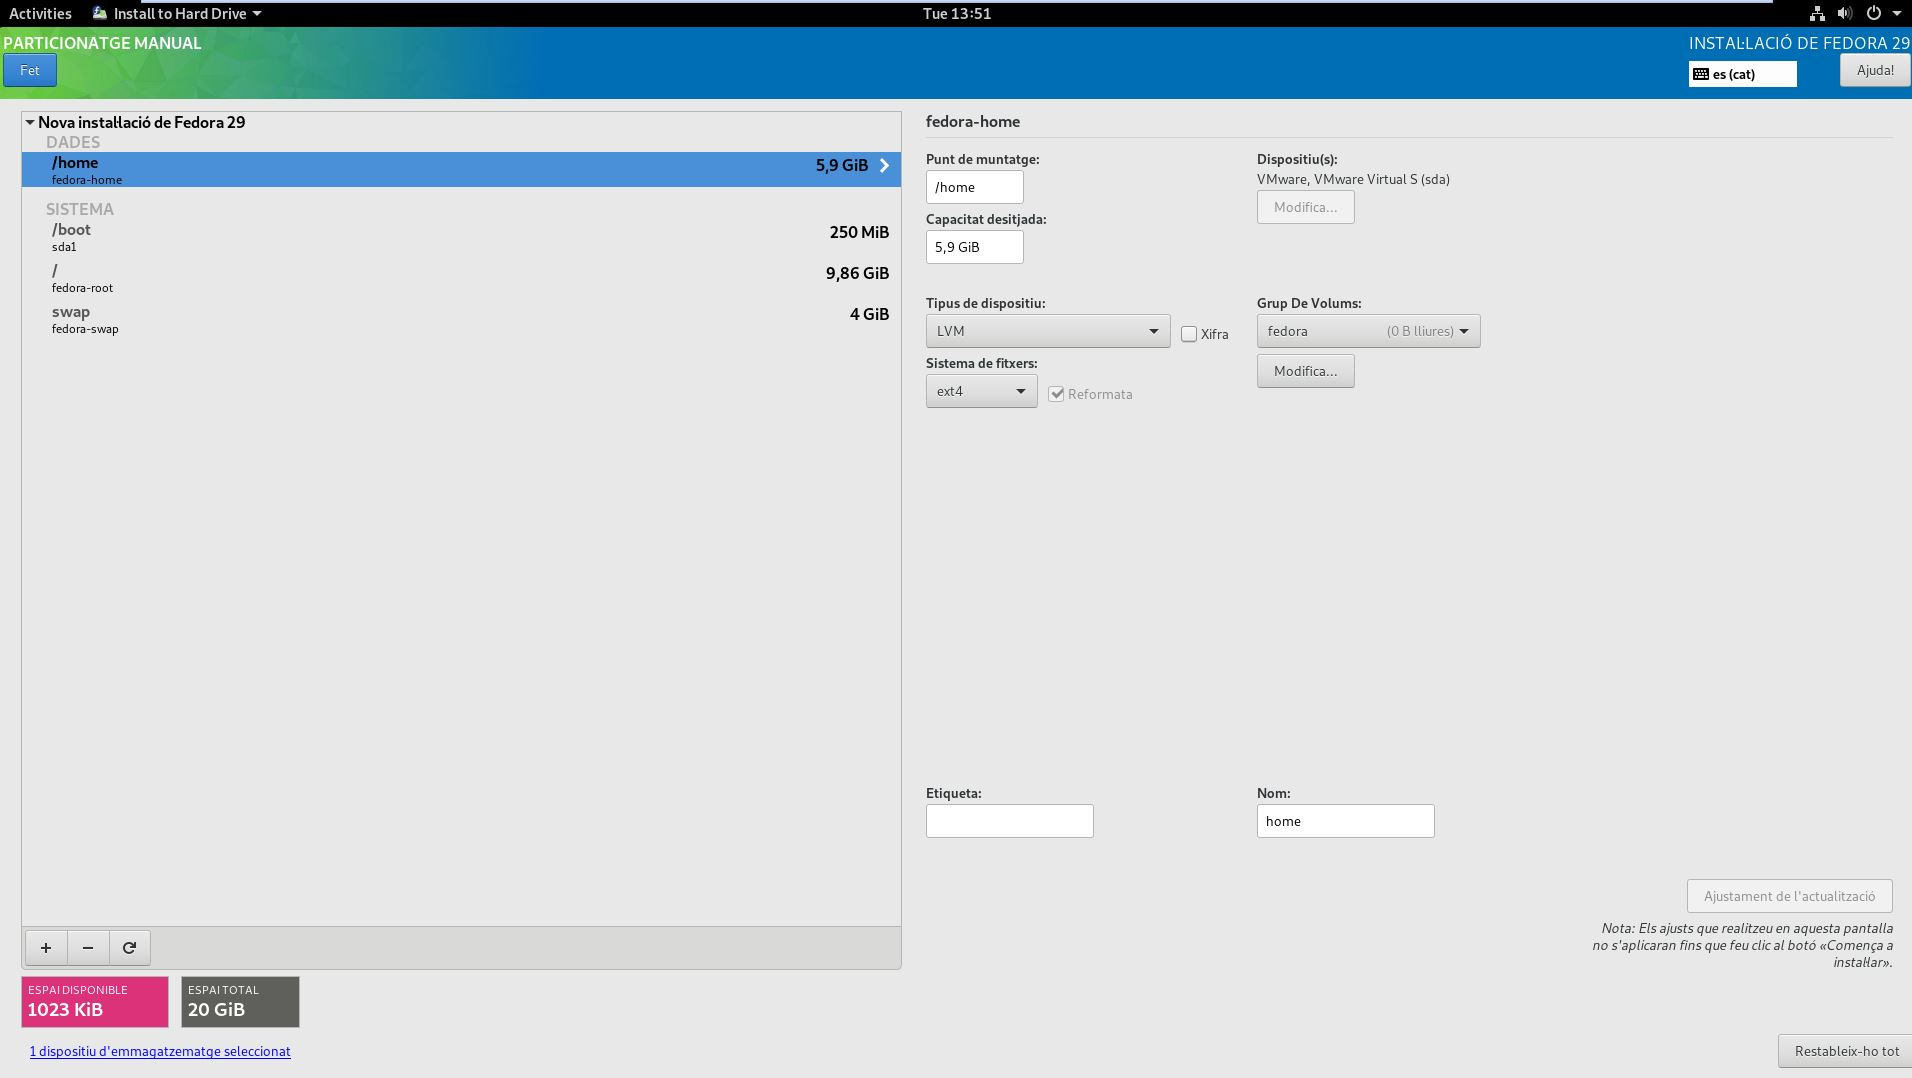
\includegraphics[width=11cm]{anex/fedora3.JPG}
    \end{center}
    \caption{Podemos configurar las particiones en el formato que queramos una partición para todo el sistema o frentes particiones para las carpetas generales}
    \begin{center}
        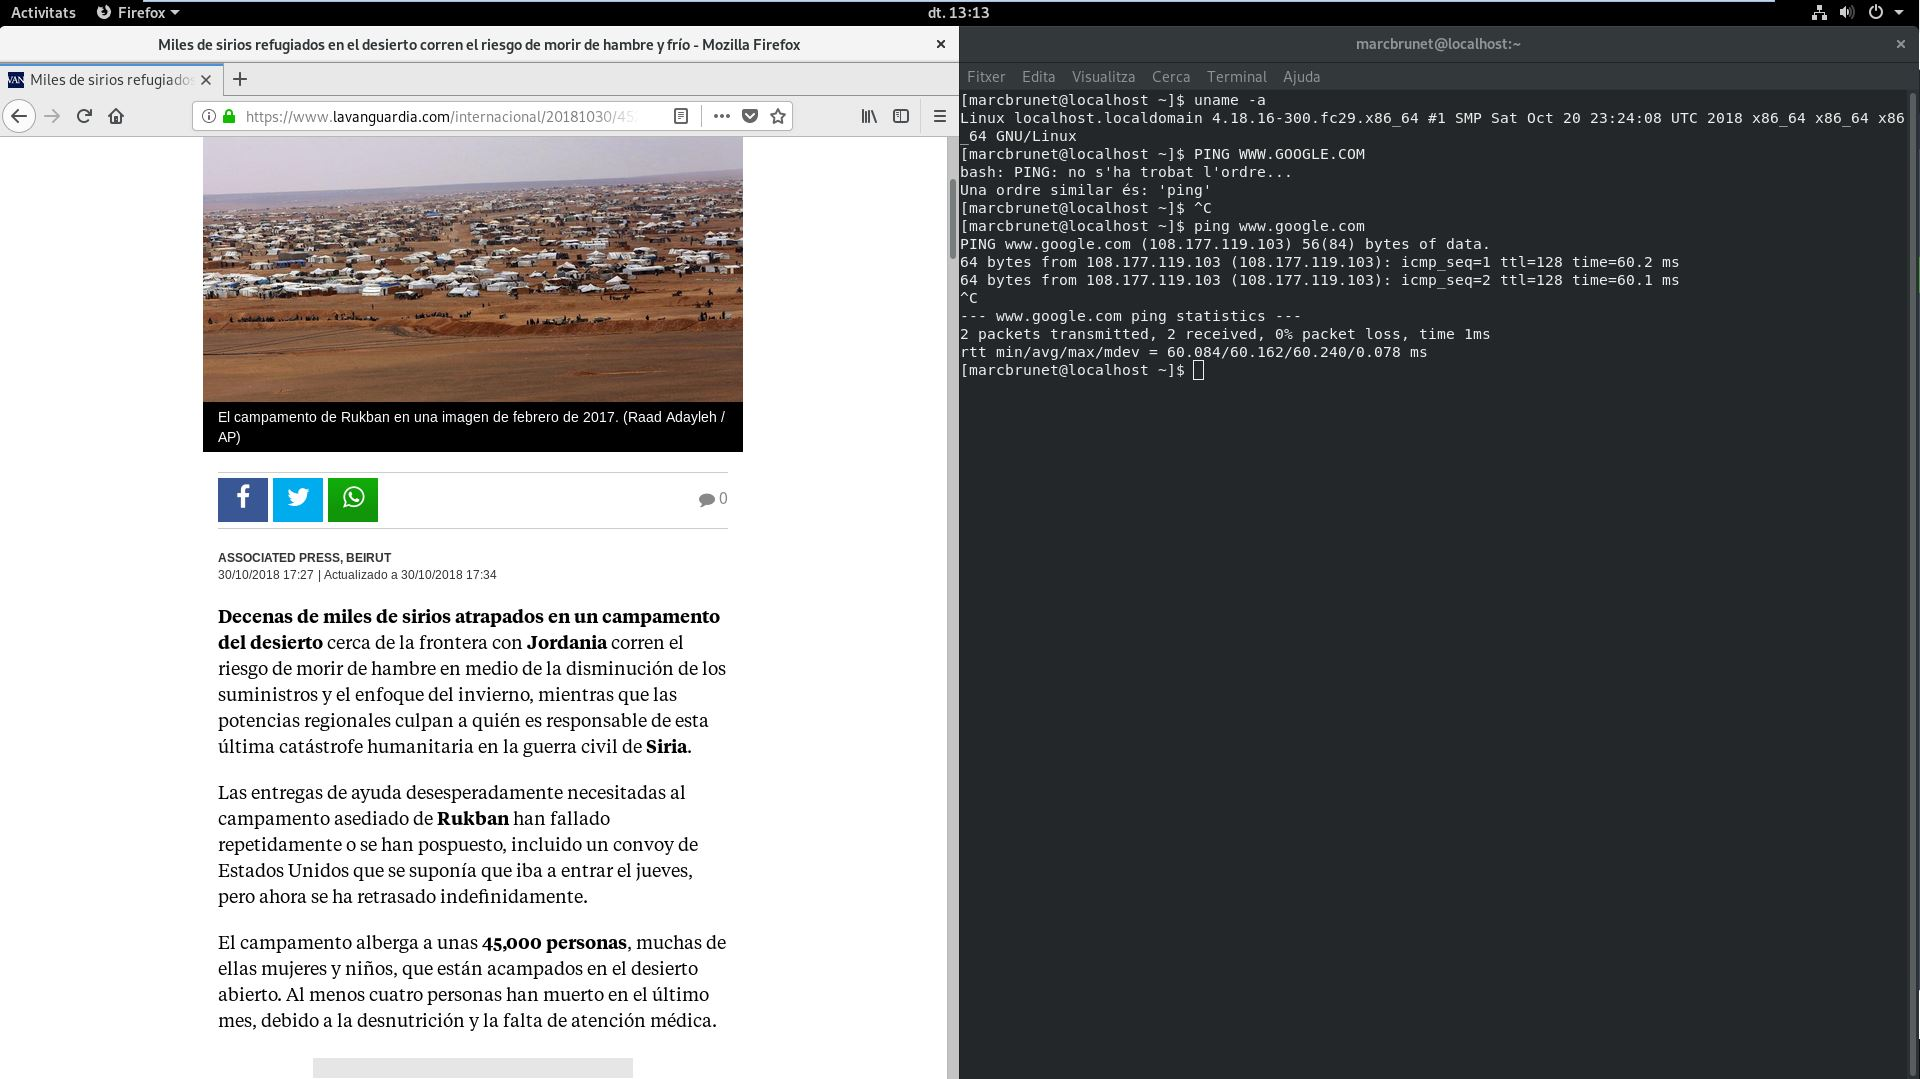
\includegraphics[width=11cm]{anex/fedora4.JPG}
    \end{center}
    \caption{Al iniciar nos pedirá la configuran del usuario y podremos comenzar a usar el sistema, ejecución del comando uname -a i ping + la vanguardia }
\end{figure}
\clearpage

\subsection{Ubtuntu}
\subsubsection{cat /etc/passwd}
\begin{lstlisting} [ basicstyle=\tiny,]
marc@ubuntu:~$ cat /etc/passwd
root:x:0:0:root:/root:/bin/bash
daemon:x:1:1:daemon:/usr/sbin:/usr/sbin/nologin
bin:x:2:2:bin:/bin:/usr/sbin/nologin
sys:x:3:3:sys:/dev:/usr/sbin/nologin
sync:x:4:65534:sync:/bin:/bin/sync
games:x:5:60:games:/usr/games:/usr/sbin/nologin
man:x:6:12:man:/var/cache/man:/usr/sbin/nologin
lp:x:7:7:lp:/var/spool/lpd:/usr/sbin/nologin
mail:x:8:8:mail:/var/mail:/usr/sbin/nologin
news:x:9:9:news:/var/spool/news:/usr/sbin/nologin
uucp:x:10:10:uucp:/var/spool/uucp:/usr/sbin/nologin
proxy:x:13:13:proxy:/bin:/usr/sbin/nologin
www-data:x:33:33:www-data:/var/www:/usr/sbin/nologin
backup:x:34:34:backup:/var/backups:/usr/sbin/nologin
list:x:38:38:Mailing List Manager:/var/list:/usr/sbin/nologin
irc:x:39:39:ircd:/var/run/ircd:/usr/sbin/nologin
gnats:x:41:41:Gnats Bug-Reporting System (admin):/var/lib/gnats:/usr/sbin/nologin
nobody:x:65534:65534:nobody:/nonexistent:/usr/sbin/nologin
systemd-network:x:100:102:systemd Network Management,,,:/run/systemd/netif:/usr/sbin/nologin
systemd-resolve:x:101:103:systemd Resolver,,,:/run/systemd/resolve:/usr/sbin/nologin
syslog:x:102:106::/home/syslog:/usr/sbin/nologin
messagebus:x:103:107::/nonexistent:/usr/sbin/nologin
_apt:x:104:65534::/nonexistent:/usr/sbin/nologin
uuidd:x:105:111::/run/uuidd:/usr/sbin/nologin
avahi-autoipd:x:106:112:Avahi autoip daemon,,,:/var/lib/avahi-autoipd:/usr/sbin/nologin
usbmux:x:107:46:usbmux daemon,,,:/var/lib/usbmux:/usr/sbin/nologin
dnsmasq:x:108:65534:dnsmasq,,,:/var/lib/misc:/usr/sbin/nologin
rtkit:x:109:114:RealtimeKit,,,:/proc:/usr/sbin/nologin
cups-pk-helper:x:110:116:user for cups-pk-helper service,,,:/home/cups-pk-helper:/usr/sbin/nologin
speech-dispatcher:x:111:29:Speech Dispatcher,,,:/var/run/speech-dispatcher:/bin/false
whoopsie:x:112:117::/nonexistent:/bin/false
kernoops:x:113:65534:Kernel Oops Tracking Daemon,,,:/:/usr/sbin/nologin
saned:x:114:119::/var/lib/saned:/usr/sbin/nologin
pulse:x:115:120:PulseAudio daemon,,,:/var/run/pulse:/usr/sbin/nologin
avahi:x:116:122:Avahi mDNS daemon,,,:/var/run/avahi-daemon:/usr/sbin/nologin
colord:x:117:123:colord colour management daemon,,,:/var/lib/colord:/usr/sbin/nologin
hplip:x:118:7:HPLIP system user,,,:/var/run/hplip:/bin/false
geoclue:x:119:124::/var/lib/geoclue:/usr/sbin/nologin
gnome-initial-setup:x:120:65534::/run/gnome-initial-setup/:/bin/false
gdm:x:121:125:Gnome Display Manager:/var/lib/gdm3:/bin/false
marc:x:1000:1000:marc,,,:/home/marc:/bin/bash

        \end{lstlisting}
        
        \subsubsection{cat /etc/group}
\begin{lstlisting} [ basicstyle=\tiny,]
root:x:0:
daemon:x:1:
bin:x:2:
sys:x:3:
adm:x:4:syslog,marc
tty:x:5:
disk:x:6:
lp:x:7:
mail:x:8:
news:x:9:
uucp:x:10:
man:x:12:
proxy:x:13:
kmem:x:15:
dialout:x:20:
fax:x:21:
voice:x:22:
cdrom:x:24:marc
floppy:x:25:
tape:x:26:
sudo:x:27:marc
audio:x:29:pulse
dip:x:30:marc
www-data:x:33:
backup:x:34:
operator:x:37:
list:x:38:
irc:x:39:
src:x:40:
gnats:x:41:
shadow:x:42:
utmp:x:43:
video:x:44:
sasl:x:45:
plugdev:x:46:marc
staff:x:50:
games:x:60:
users:x:100:
nogroup:x:65534:
systemd-journal:x:101:
systemd-network:x:102:
systemd-resolve:x:103:
input:x:104:
crontab:x:105:
syslog:x:106:
messagebus:x:107:
netdev:x:108:
mlocate:x:109:
ssl-cert:x:110:
uuidd:x:111:
avahi-autoipd:x:112:
bluetooth:x:113:
rtkit:x:114:
ssh:x:115:
lpadmin:x:116:marc
whoopsie:x:117:
scanner:x:118:saned
saned:x:119:
pulse:x:120:
pulse-access:x:121:
avahi:x:122:
colord:x:123:
geoclue:x:124:
gdm:x:125:
marc:x:1000:
sambashare:x:126:marc
\end{lstlisting}

\clearpage
\subsection{Fedora}
\subsubsection{cat /etc/passwd}
\begin{lstlisting} [ basicstyle=\tiny,]
[marc@localhost ~]$ cat /etc/passwd
root:x:0:0:root:/root:/bin/bash
bin:x:1:1:bin:/bin:/sbin/nologin
daemon:x:2:2:daemon:/sbin:/sbin/nologin
adm:x:3:4:adm:/var/adm:/sbin/nologin
lp:x:4:7:lp:/var/spool/lpd:/sbin/nologin
sync:x:5:0:sync:/sbin:/bin/sync
shutdown:x:6:0:shutdown:/sbin:/sbin/shutdown
halt:x:7:0:halt:/sbin:/sbin/halt
mail:x:8:12:mail:/var/spool/mail:/sbin/nologin
operator:x:11:0:operator:/root:/sbin/nologin
games:x:12:100:games:/usr/games:/sbin/nologin
ftp:x:14:50:FTP User:/var/ftp:/sbin/nologin
nobody:x:65534:65534:Kernel Overflow User:/:/sbin/nologin
dbus:x:81:81:System message bus:/:/sbin/nologin
systemd-coredump:x:999:997:systemd Core Dumper:/:/sbin/nologin
systemd-network:x:192:192:systemd Network Management:/:/sbin/nologin
systemd-resolve:x:193:193:systemd Resolver:/:/sbin/nologin
tss:x:59:59:Account used by the trousers package to sandbox the tcsd daemon:/dev/null:/sbin/nologin
polkitd:x:998:996:User for polkitd:/:/sbin/nologin
gluster:x:997:994:GlusterFS daemons:/run/gluster:/sbin/nologin
rtkit:x:172:172:RealtimeKit:/proc:/sbin/nologin
pulse:x:171:171:PulseAudio System Daemon:/var/run/pulse:/sbin/nologin
qemu:x:107:107:qemu user:/:/sbin/nologin
nm-openconnect:x:996:990:NetworkManager user for OpenConnect:/:/sbin/nologin
unbound:x:995:989:Unbound DNS resolver:/etc/unbound:/sbin/nologin
usbmuxd:x:113:113:usbmuxd user:/:/sbin/nologin
chrony:x:994:988::/var/lib/chrony:/sbin/nologin
geoclue:x:993:987:User for geoclue:/var/lib/geoclue:/sbin/nologin
avahi:x:70:70:Avahi mDNS/DNS-SD Stack:/var/run/avahi-daemon:/sbin/nologin
pipewire:x:992:986:PipeWire System Daemon:/var/run/pipewire:/sbin/nologin
saslauth:x:991:76:Saslauthd user:/run/saslauthd:/sbin/nologin
dnsmasq:x:985:985:Dnsmasq DHCP and DNS server:/var/lib/dnsmasq:/sbin/nologin
radvd:x:75:75:radvd user:/:/sbin/nologin
rpc:x:32:32:Rpcbind Daemon:/var/lib/rpcbind:/sbin/nologin
openvpn:x:984:982:OpenVPN:/etc/openvpn:/sbin/nologin
nm-openvpn:x:983:981:Default user for running openvpn spawned by NetworkManager:/:/sbin/nologin
abrt:x:173:173::/etc/abrt:/sbin/nologin
apache:x:48:48:Apache:/usr/share/httpd:/sbin/nologin
colord:x:982:980:User for colord:/var/lib/colord:/sbin/nologin
rpcuser:x:29:29:RPC Service User:/var/lib/nfs:/sbin/nologin
gdm:x:42:42::/var/lib/gdm:/sbin/nologin
gnome-initial-setup:x:981:979::/run/gnome-initial-setup/:/sbin/nologin
sshd:x:74:74:Privilege-separated SSH:/var/empty/sshd:/sbin/nologin
vboxadd:x:980:1::/var/run/vboxadd:/sbin/nologin
tcpdump:x:72:72::/:/sbin/nologin
marc:x:1000:1000:marc:/home/marc:/bin/bash

\end{lstlisting}
    
        
\subsubsection{cat /etc/group}
\begin{lstlisting} [ basicstyle=\tiny,]
root:x:0:
bin:x:1:
daemon:x:2:
sys:x:3:
adm:x:4:
tty:x:5:
disk:x:6:
lp:x:7:
mem:x:8:
kmem:x:9:
wheel:x:10:marc
cdrom:x:11:
mail:x:12:
man:x:15:
dialout:x:18:
floppy:x:19:
games:x:20:
tape:x:33:
video:x:39:
ftp:x:50:
lock:x:54:
audio:x:63:
users:x:100:
nobody:x:65534:
dbus:x:81:
utmp:x:22:
utempter:x:35:
input:x:999:
kvm:x:36:qemu
render:x:998:
systemd-journal:x:190:
systemd-coredump:x:997:
systemd-network:x:192:
systemd-resolve:x:193:
tss:x:59:
polkitd:x:996:
dip:x:40:
printadmin:x:995:
gluster:x:994:
rtkit:x:172:
pulse-access:x:993:
pulse-rt:x:992:
pulse:x:171:
brlapi:x:991:
qemu:x:107:
nm-openconnect:x:990:
unbound:x:989:
usbmuxd:x:113:
chrony:x:988:
geoclue:x:987:
avahi:x:70:
pipewire:x:986:
saslauth:x:76:
dnsmasq:x:985:
radvd:x:75:
rpc:x:32:
ssh_keys:x:984:
libvirt:x:983:
openvpn:x:982:
nm-openvpn:x:981:
abrt:x:173:
apache:x:48:
colord:x:980:
rpcuser:x:29:
gdm:x:42:
gnome-initial-setup:x:979:
sshd:x:74:
slocate:x:21:
vboxsf:x:978:
tcpdump:x:72:
marc:x:1000:

\end{lstlisting}
\end{document}